	\documentclass[12pt,a4paper,titlepage,openany]{report}
\usepackage{zakljucna_FAMNIT_1_stopnja_MA_MEF_EN_2016}
\usepackage{enumitem}  
% Head of document:

\fancyhf{}
\lhead[]{{\fontsize{9.3}{12}\selectfont
Avdullahu A. Representations of graphs as induced subgraphs of Hamming graphs.\\
\noindent Univerza na Primorskem, Fakulteta za matematiko, naravoslovje in informacijske tehnologije, year}}
\chead[]{\fancyplain{}{}}
\rhead[]{\fancyplain{\thepage}
{\thepage}}
\cfoot[]{\fancyplain{}{}}
\lfoot[]{\fancyplain{}{}}
\rfoot[]{\fancyplain{}{}}
\normalsize

%%%%%%%%%%%%%%%%%%%%%%%%% BEGINNING OF DOCUMENT %%%%%%%%%%%%%%%%%%%%%%%%%%%%%%%%%%%%%%%%%%5

%%%%%%%%%%%%%%%%%%%%%%%%% Title page %%%%%%%%%%%%%%%%%%%%%%%%%


\begin{document}
\pagenumbering{Roman}
\pagestyle{empty}
\begin{center}
\noindent \large UNIVERZA NA PRIMORSKEM\\
\large FAKULTETA ZA MATEMATIKO, NARAVOSLOVJE IN\\
INFORMACIJSKE TEHNOLOGIJE


\normalsize
\vspace{5.5cm}
Seminar - uvod v raziskovalno delo\\
(Seminar - Introduction to Research Work)\\
\textbf{\large Naslov seminarske naloge}\\
\normalsize
(Representations of graphs as induced subgraphs of Hamming graphs)\\
\end{center}

\begin{flushleft}
\vspace{5cm}
\noindent Ime in priimek: Arber Avdullahu
% add your first name and last name in the line above
\\
\noindent \v Studijski program: Matematika
% add your study program in the line above
\\
\noindent Mentor: dr. Martin Milani\v c
% add the academic title, first name, and last name of your mentor in the line above
\\
\noindent Somentor: dr. Marcelo Mydlarz
% if you have a co-mentor, add his/her academic title, first name, and last name in the line above
% if you do not have a co-mentor, delete the line above and the line below
\\
\end{flushleft}

\vspace{4cm}
\begin{center}
\large \textbf{Koper, April 2019}
% add the month and year of submission of your final project paper
\end{center}
\newpage

\pagestyle{fancy}
%%%%%%%%%%%%%%%%%%%%%%%%%%%%%%% Key words documentation (Slovene and English) %%%%%%%%%%%

\section*{Klju\v cna dokumentacijska informacija}

\medskip
\begin{center}
\fbox{\parbox{\linewidth}{
\vspace{0.2cm}
\noindent
Ime in PRIIMEK:\vspace{0.5cm}\\
Naslov seminarske naloge:\vspace{0.5cm}\\
Kraj:\vspace{0.5cm}\\
Leto:\vspace{0.5cm}\\
\v Stevilo listov: \hspace{2cm} \v Stevilo slik: \hspace{2.6cm} \v Stevilo tabel:\hspace{2cm}\vspace{0.5cm}\\
\v Stevilo prilog: \hspace{1.9cm} \v Stevilo strani prilog: \hspace{1cm} \v Stevilo referenc:\vspace{0.5cm}\\
Mentor:\vspace{0.5cm}\\
Somentor:\vspace{0.5cm}\\
Klju\v cne besede:\vspace{0.5cm}\\
Math.~Subj.~Class.~(2010):\vspace{0.5cm}\\
{\bf Izvle\v cek:}\\
Izvle\v cek predstavlja kratek, a jedrnat prikaz vsebine naloge. V najve\v c 250 besedah naka\v zemo problem, metode, rezultate, klju\v cne ugotovitve in njihov pomen.
\vspace{0.2cm}
}}
\end{center}

\newpage

\section*{Key words documentation}

\medskip

\begin{center}
\fbox{\parbox{\linewidth}{
\vspace{0.2cm}
\noindent
Name and SURNAME:\vspace{0.5cm}\\
Title of term project paper:\vspace{0.5cm}\\
Place:\vspace{0.5cm}\\
Year:\vspace{0.5cm}\\
Number of pages:\hspace{1.6cm} Number of figures:\hspace{2.2cm} Number of tables:\vspace{0.5cm}\\
Number of appendices:\hspace{0.6cm} Number of appendix pages:\hspace{0.8cm}Number of references:\vspace{0.5cm}\\
Mentor: title~First Name~Last Name, PhD\vspace{0.5cm}\\
% for : "title" write one of the following:
% Assist.~Prof.~(if the title is "docent"),
% Assoc.~Prof.~(if the title is "izredni profesor"),
% Prof.~(if the title is "profesor")
Co-Mentor:\vspace{0.5cm}\\
Keywords:\vspace{0.5cm}\\
Math.~Subj.~Class.~(2010):\vspace{0.5cm}\\
{\bf Abstract:}
\vspace{0.2cm}
}}
\end{center}




%%%%%%%%%%%%%%%%%%%%%%%%%%%%%%% Acknowledgement %%%%%%%%%%%%%%%%%%%%%%%%%%%%%%%%%%%%%

\newpage
\section*{Acknowledgement}

Here we thank all involved with our term project paper, that is, persons or institutions that helped us in our work and/or made it possible.
We can also thank the mentor and the co-mentor (if there is one)

%%%%%%%%%%%%%%%%%%%%%%%%%%%%% Table of contents, list of figures, etc. %%%%%%%%%%%%%%%%%%%%%%%%%%%%%%
\newpage

\tableofcontents
\addtocontents{toc}{\protect\thispagestyle{fancy}}
% if there are no tables in your final project paper, delete the following three lines
\newpage
\listoftables
\addtocontents{lot}{\protect\thispagestyle{fancy}}
% if there are no figures in your final project paper, delete the following three lines
\newpage
\listoffigures
\addtocontents{lof}{\protect\thispagestyle{fancy}}
\newpage
% Since the appendices are not numbered, we also do not want to show the dots to their (non-existing) page numbers.
\renewcommand{\cftdot}{}
\listofappendices
\thispagestyle{fancy}
\newpage

\chapter*{List of Abbreviations}
\thispagestyle{fancyplain}
\begin{longtable}{@{}p{1cm}@{}p{\dimexpr\textwidth-1cm\relax}@{}}
\nomenclature{{\it i.e.}}{that is}
\nomenclature{{\it e.g.}}{for example}
\end{longtable}
\newpage

\normalsize

%%%%%%%%%%%%%%%%%%%%%%%%%%%%%%%%%% Chapters: %%%%%%%%%%%%%%%%%%%%%%%%%%%%%%%%%%%%%

% Hint: You might find it convenient to keep the contents of separate chapters in separate files, each in their own
% .tex file. They all have to be stored in the same folder as the main file. Each chapter is included with the \include command.
% Example: we can insert FirstChapter.tex and SecondChapter.tex as follows:
% \include{FirstChapter}
% \include{SecondChapter}

\chapter{Introduction}
\thispagestyle{fancy}
\pagenumbering{arabic}

How difficult is it to determine if
a given graph $G$ can be realized in $\mathbb{R}^d$ so that vertices are mapped to distinct points and two vertices are adjacent if and only if the corresponding points are on a common line that is parallel to some axis? Let us refer to any such mapping as a d-realization of $G$ and say that a graph is $d$-realizable if it has a $d$-realization.The class of $d$-realizable graphs was studied
in the literature for decades, under diverse names such as arrow graphs (Cook, 1974), $(d - 1)$-plane graphs and $(d -1)$-line graphs of $d$-partite $d$-uniform hypergraphs (Bermond etal., 1977), $d$-dimensional cellular graphs (Gurvich and Temkin, 1992), $d$-dimensional chessboard graphs (Staton and  Wingard, 1998), and d-dimensional gridline graphs (Peterson, 2003).\newline
In order to determine how hard will it be to answer that question we should first take a look at the following definitions:\newline
Let $A$ be an algorithm that solves a problem $\mathcal{P}$. The running time of algorithm $A$ is the number of basic calculation steps performed by $A$ (additions, subtractions, multiplications, comparison of two numbers, etc.). The time complexity of algorithm $A$ is the function $T_A(n)$ that
measures the running time of $A$ in the worst case:
\begin{center}
	$T_A : n \rightarrow $ largest running time of $A$ on input instances of size $\leq$ $n$.
\end{center} 

Given two functions $f,g : \mathbb{N} \to \mathbb{N}$, we say that $f$ is of order (at most) $O(g)$ if there exists a constant $C > 0$ such that $f(n) \leq C\cdot g(n)$ for all $n \in \mathbb{N}$ and we write $f = O(g)$.\newline
An algorithm $A$ is \textit{polynomial} if its time complexity $T_A(n)$ is of order $O(n^k)$ for some $k \in \mathbb{N}$.
Polynomial algorithms are also said to be efficient.

A \textit{decision problem} is a problem in which the set of instances divides into two sets depending on whether the answer is YES or NO.
In computational complexity theory, the following three classes of decision problem are of interest:
\begin{itemize}
\item {\it P} is the set of decision problems that can be solved by a polynomial algorithm. Intuitively: $P$ is the set of problems that can be solved efficiently.
\item {\it NP} is the set of decision problems with the following property:
If the answer is YES then there exists a certificate that
enables us to verify this fact in polynomial time. Intuitively: NP is the set of problems for which we can
quickly verify a positive answer if we are given a solution.
\item {\it co-NP} is the set of decision problems with the following property:
If the answer is NO then there exists a certificate that
enables us to verify this fact in polynomial time.
\end{itemize}


Recently, Sangha and Zito studied $d$-realizable graphs in the more general context of the so-called Line-of-Sight (LoS) networks [49]. Line of Sight (LoS) networks provide a model of wireless communication which incorporates visibility constraints. Vertices of such networks can be embedded in finite $d$-dimensional grids of size $n$, and two vertices are adjacent if they share a line of sight and are at distance less than $\omega$ where two points $x=(x_1, \ldots,x_d)$ and $x'=(x_1',\ldots ,x_d')$ share a line of sight if there exists some $j\in \{1,\ldots,d\}$ such that $x_i=x_i'$ for all $i\in \{1,\ldots,d\} \symbol{92} \{j\}$. They studied large independent sets in LoS networks. They proved that the computational problem of finding a largest independent set can be solved optimally in polynomial time for one dimensional LoS networks. However, for $d \geq 2$, the (decision version of) the problem becomes NP-hard for any fixed $\omega \geq 3$ and even if $ω$ is chosen to be a
function of $n$ that is $O(n^{1-\epsilon})$ for any fixed $\epsilon>0$. In addition they showed that the problem is also NP-hard when $\omega = n$ for $d \geq 3$. This result
extends earlier work which showed that the problem is solvable in polynomial time for gridline graphs when $d = 2$.\newline
For the small-dimensional cases, $d \in \{2, 3\}$, Peterson suggested an application of $d$-realizable graphs to robotics [46]: if the movement of a robot is restricted to be along axis-parallel directions only and turns are
allowable only at certain points, then a shortest path in a $d$-realized graph gives the number of turns required.



Despite many studies on $d$-realizable graphs in the literature, determining the computational complexity of recognizing $d$-realizable graphs has been elusive except for $d \in \{1, 2\}$,
when $d$-realizable graphs coincide with complete graphs and with line graphs of bipartite graphs, respectively (and can be recognized in polynomial time).The problem that we study in this final project paper is to analyze the question about recognition complexity of $d$-realizable graphs for $d \geq 3$, asked explicitly by Peterson in 2003 [46].
We show that for all $d \geq 3$, determining if a given graph is $d$-realizable is {\it NP}-complete, even for bipartite graphs.We also identify some tractable cases.
We present the work of Martin Milani\v c, Peter Mur\v si\v c, and Marcelo Mydlarz $d$-realizable graphs (for any positive integer $d$) in the class of $HHD$-free graphs, a large class of perfect graphs containing chordal graphs and distance-hereditary graphs. The characterization leads to a linear time recognition algorithm.\newline

My approach is based on the fact that a graph $G$ is $d$ -realizable if and only if $G$ is an induced subgraph of a Cartesian product of $d$ complete graphs. Given two graphs G and H, their Cartesian product is the graph $G\square H$ with vertex set $V (G) \times V (H)$ in which two
vertices $(u_1 , u_2 )$ and $(v_1 , v_2 )$ are adjacent if and only if either $u_1 v_1\in E(G)$ and $u_2 = v_2$ ,
or $u_1 = v_1$ and $u_2 v_2 \in E(H)$. The Cartesian product is associative and commutative (in the sense that $G\square H \cong H\square G$ where $\cong$ denotes the graph isomorphism relation). Another
name for Cartesian products of complete graphs is Hamming graphs; a Hamming graph is $d$-dimensional if it is the Cartesian product of $d$ nontrivial complete graphs. The 3-dimensional Hamming graphs having all factors of the same size were studied in the literature under the name cubic lattice graphs [37, 12, 11, 1, 16], hence, 3-realizable graphs are exactly the induced subgraphs of cubic lattice graphs. Results are based on a characterization of induced subgraphs of d-dimensional Hamming graphs due to Klav\v zar and Peterin [33], expressed in terms of the existence of a particular edge labeling. For the 3-dimensional case, we develop a more specific characterization based on induced cycles of the graph and use it to prove hardness of recognizing 3-realizable graphs via a reduction from the 3-edge-coloring problem
in cubic graphs. The hardness of the 3-dimensional case forms the basis for establishing hardness for all higher dimensions.\newline

Since a $d$-realizable graph is also $(d + 1)$-realizable, the notion of d-realizability suggests a natural graph parameter. The Cartesian dimension of a graph $G = (V, E)$, denoted $Cdim(G)$, is defined as the minimum non-negative integer $d$ such that $G$ is $d$-realizable, if such an integer exists, and $\infty$, otherwise. The infinite case can indeed occur, even some small graphs – the diamond, the 5-cycle, and the complete bipartite graph $K_{2,3}$ , for example – cannot be realized in any dimension. Note that $Cdim(G)$, when finite and strictly positive, is the minimum positive integer $d$ such that $G$ is an induced subgraph of the Cartesian product
of $d$ complete graphs. This point of view adds the Cartesian dimension of a graph to the list of graph dimensions studied in the literature related to various embeddings of graphs into Cartesian product graphs [24, 20, 27, 34]. Other dimensions were studied related to the
strong product [22, 15, 32, 47] and the direct product of graphs [41, 48].

\chapter{Preliminaries}
\thispagestyle{fancy}

In this chapter we will talk about necessary and sufficent conditions for a graph to be an induced subgraph of a Hamming graph and some results regarding those conditions. 

\chapter{Characterizing Subgraphs of Hamming Graphs}
\thispagestyle{fancy}

In this chapter we will talk about necessary and sufficent conditions for a graph to be an induced subgraph of a Hamming graph and some results regarding those conditions.  

\section{KP-labeling}\label{kp-labeling-section}
We take a closer look at the characterization of induced subgraphs of Hamming graphs due to Klav\v zar and Peterin. \newline
Before going to the result we need to go through couple of definitions and some results.
\newline
\begin{lemma}\label{cutedgecycle}
An edge $e = \{u, v\}$ of a graph G is a cut-edge if and only if it does not belong to any cycle.
\end{lemma}
\begin{proof} Take any edge $e = \{u, v\}$. Remove this edge from our graph: if the graph is still connected, then there is some path from $u$ to $v$ not involving $e$;
consequently, if we add $e$ to the end of this path, we get a cycle. Thus, if $e$ is not a cut-edge, then $e$ belongs to a cycle.\newline
Conversely, suppose that $e = \{u, v\}$ lies in a cycle.
Let $P$ be the path from $u$ to $v$ that does not use $e$ (i.e. goes the other way around the cycle.) Pick any $x, y$ in $G$; because $G$ is connected, there is a path from $x$ to $y$ in $G$. Take this path, and edit it as follows:
whenever the edge $e$ shows up, replace this with the path $P$ (or $P$ traced backwards, if needed.) This then creates a walk from $x$ to $y$; by deleting cycles if necessary, this walk can be turned into a path from $x$ to $y$, and thus $G-e$ is connected. So if $e$ is contained in a cycle, it’s not a cut-edge.
\end{proof}
The Cartesian product $G\square H$ of graphs $G$ and $H$ is the graph with vertex set $V(G)\times V(H)$ in which a vertex $(a,x)$ is adjacent to a vertex $(b,y)$ whenever
$ab\in E(G)$ and $x=y$, or $a=b$ and $xy\in E(H)$. For a fixed vertex $a$ of $G$, the vertices $\{(a,x)|x\in V(H)\}$ induce a subgraph of $G \square H$ isomorphic to $H$, called an \textit{$H$-layer} of $G \square H$. Analogously we define \textit{$G$-layers}. A subgraph of $G \square H$ is called non-trivial if it intersects at least two $G$-layers and at least two $H$-layers. \newline
The map $p_G:V(G\square H) \to G$ defined by $p_G(a,x)=a$, is called a projection. The image of an edge $(a,x)(b,y)$ under a projection is an edge when $x=y$ or a vertex in when $a=b$.\newline
\begin{figure}\label{fig:cartProduct}
\centering
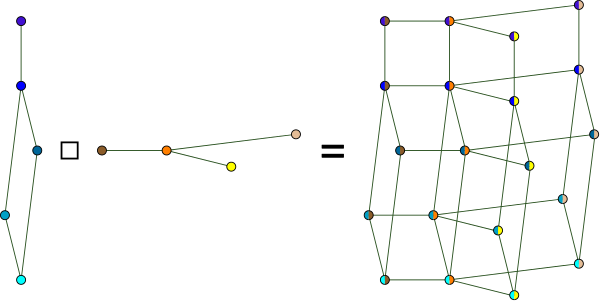
\includegraphics[scale=0.45]{figures/Graph-Cartesian-product.png}
\caption{The Cartesian product of graphs.}

\end{figure}
Cartesian products of complete graphs are known as Hamming graphs. But they can be described also as follows. For
$i=1,2,\ldots, n$ let $r_i\geq 2$ be given integers. Let $G$ be the graph whose vertices are the $n$-tuples $b_1b_2\cdots b_n$ with $b_i\in \{0,1,\ldots r_i-1\}$. Two vertices are adjacent if the corresponding tuples differ in precisely one coordinate. The vertex set of $G$ is the same as that of $K_{r_1}\square K_{r_2}\square \ldots \square K_{r_n}$ and edges in $K_{r_1}\square K_{r_2}\square \ldots \square K_{r_n}$ between two vertices are exactly those that have same vertex in every graph $K_{r_i}$ but one and since in complete graphs we have every possible edge, then it is easy to see that $G$ and $K_{r_1}\square K_{r_2}\square \ldots \square K_{r_n}$ are isomorphic. For an edge $uv$ of
$H=K_{r_1}\square K_{r_2}\square \ldots \square K_{r_n}$ we define the color map $c:E(H)\rightarrow \{1,2,\ldots n\}$ with $c(uv)=i$, where $u$ and $v$ differ in coordinate $i$.
\newline
Let $G$ be a connected graph and let $\mathcal{F}=\{F_1,F_2,\ldots F_k\}$ be a partition of $E(G)$. The \textit{quotient graph} $G/ F_i$ has connected components of $G\backslash F_i$ as vertices, two components $C$ and $C'$ being adjacent whenever there exists an edge of $F_i$ connecting a vertex of $C$ with a vertex of $C'$. For each $i$, define a map $f_i:V(G)\rightarrow V(G/ F_i)$ by $f_i(v)=C$, where $C$ is the component of $G\backslash F_i$ containing $v$. Then let
$$f:V(G)\to V(G/ F_1\square G/ F_2\square \ldots \square G/ F_k)$$
be the natural coordinate-wise mapping, that is
$$f(v)=(f_1(v),f_2(v),\ldots , f_k(v))$$
We call $f$ the \textit{quotient map} of $G$ with respect to $\mathfrak{F}$. Note that $f$ need not be one-to-one in general and that it is possible that some quotient graphs are the one vertex graph, an example is shown in Figure \ref{fnotonetoone}.
\begin{figure}[h]\label{fnotonetoone}
\begin{center}
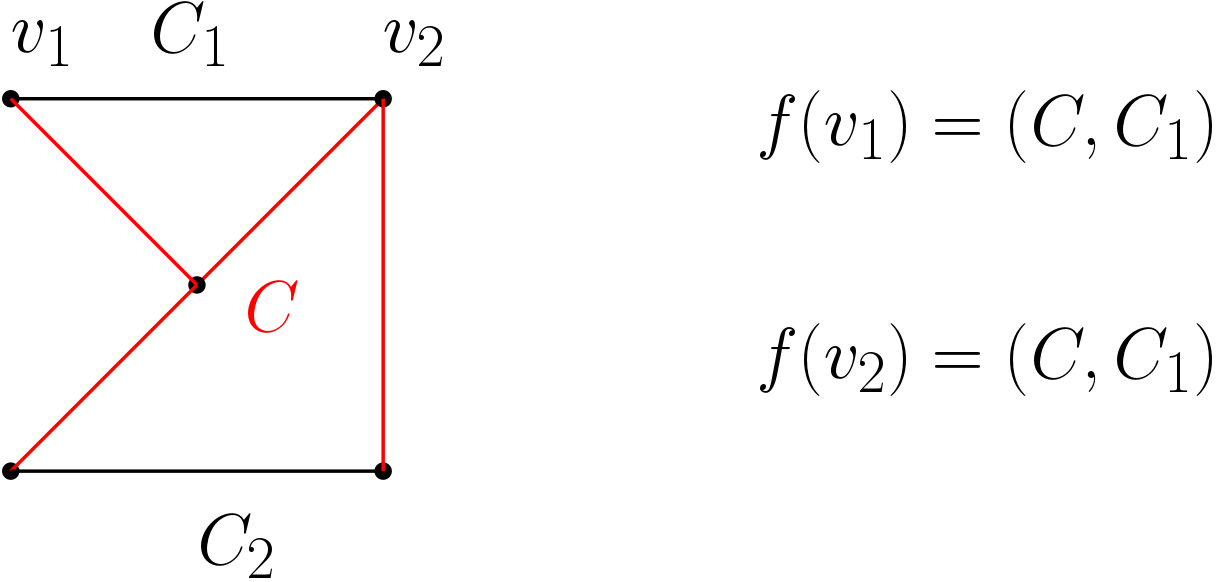
\includegraphics[width=0.8\linewidth]{figures/fnotonetoone.png}
\end{center}
\caption{An example of a graph that the quotient map is not one-to-one}
\end{figure}
 However, all the partitions $\mathfrak{F}$ introduced later will lead to one-to-one mappings with non-trivial quotient graphs.\newline
A partition $\{F_1,F_2,\ldots ,F_k\}$ of $E(G)$ naturally leads to an edge-labeling $l:E(G)\to \{1,2,\ldots,k\}$ by setting $l(e)=i$, where $e\in F_i$. Unless stated
otherwise, a labeling (or more precisely a $k$-labeling) of $G$ will mean an edge-labeling (with $k$ labels).
\newline 
Quotient graph is the central concept in this chapter, so to get a better understanding we also visualize it.
\begin{figure}[h!]
\begin{center}
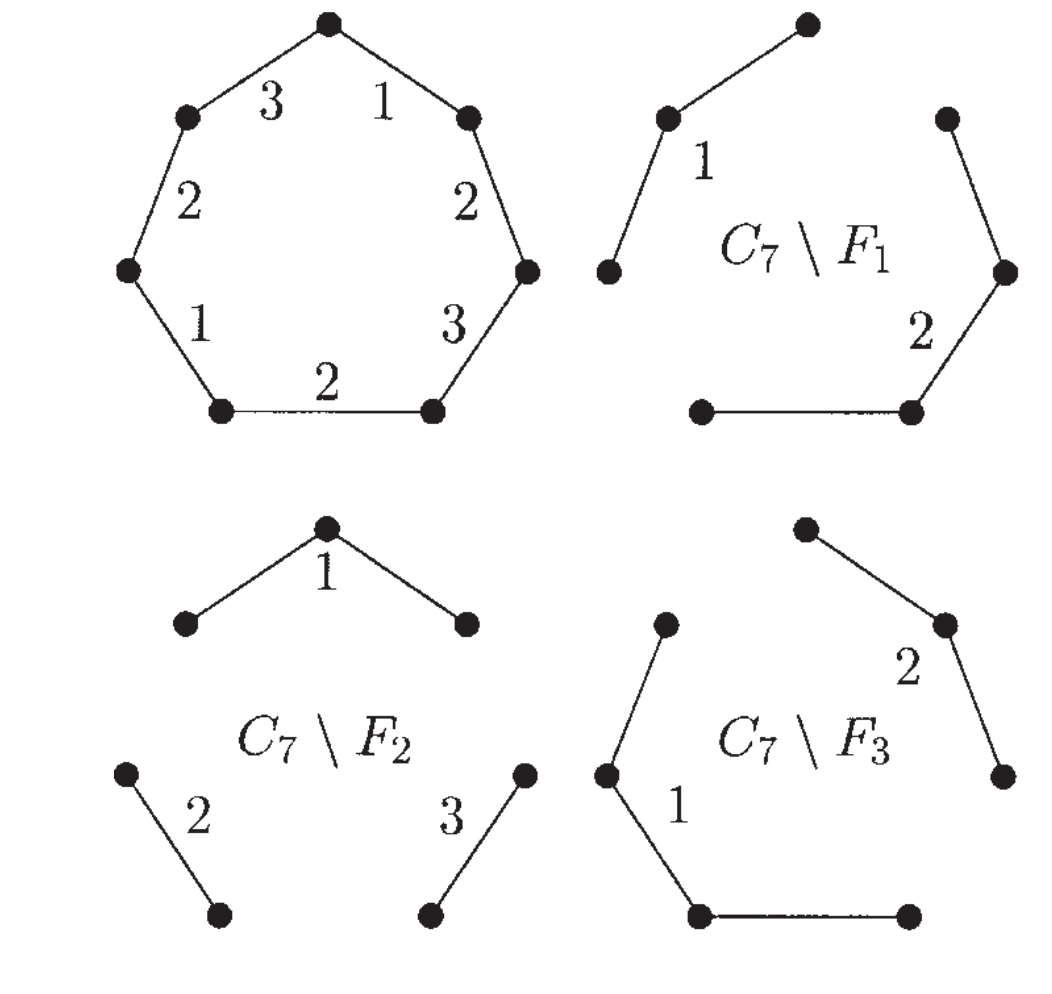
\includegraphics[width=1\linewidth]{figures/quotientgraph.png}
\end{center}
\caption{Quotient graph of $C_7$}
\end{figure}
We define the partition of $E(C_7)$ by defining $F_i$ having edges with label $i$, as we can see $C_7/ F_1$ and $C_7/F_3$ have only two vertices and since there is an edge in the correspoding $F_i$ connecting those two components, both of  $C_7\backslash F_1$ and $C_7/F_3$ are simply $K_2$, while $C_7\backslash F_2$ has three vertices but each two of compontents are connected with an edge from $F_2$ so $C_7\backslash F_2$ is simply $K_3$.   
\newline
Sandi Klav\v zar and Iztok Peterin defined two conditions to get a better understanding. They actually named them by letters $B$ and $C$, and also defined condition A which is needed for subgraphs oh Hamming graphs but since we will not need condition $A$ will name just by numbers $1$ and $2$.\newline
We say that a $d$-edge-labeling of $G$ is a ($d$-)KP-labeling if it satisfies the following conditions:
\newline
\textbf{Condition 1} The edges of any triangle have the same label.\newline
\textbf{Condition 2} Let $u$ and $v$ be arbitrary vertices of $G$ with $d_G(u,v) \geq 2$. Then there exist different labels $i$ and $j$ which both appear on any induced $u$, $v$-path.\newline
\begin{figure}[h!]\label{kpexample}
\begin{center}
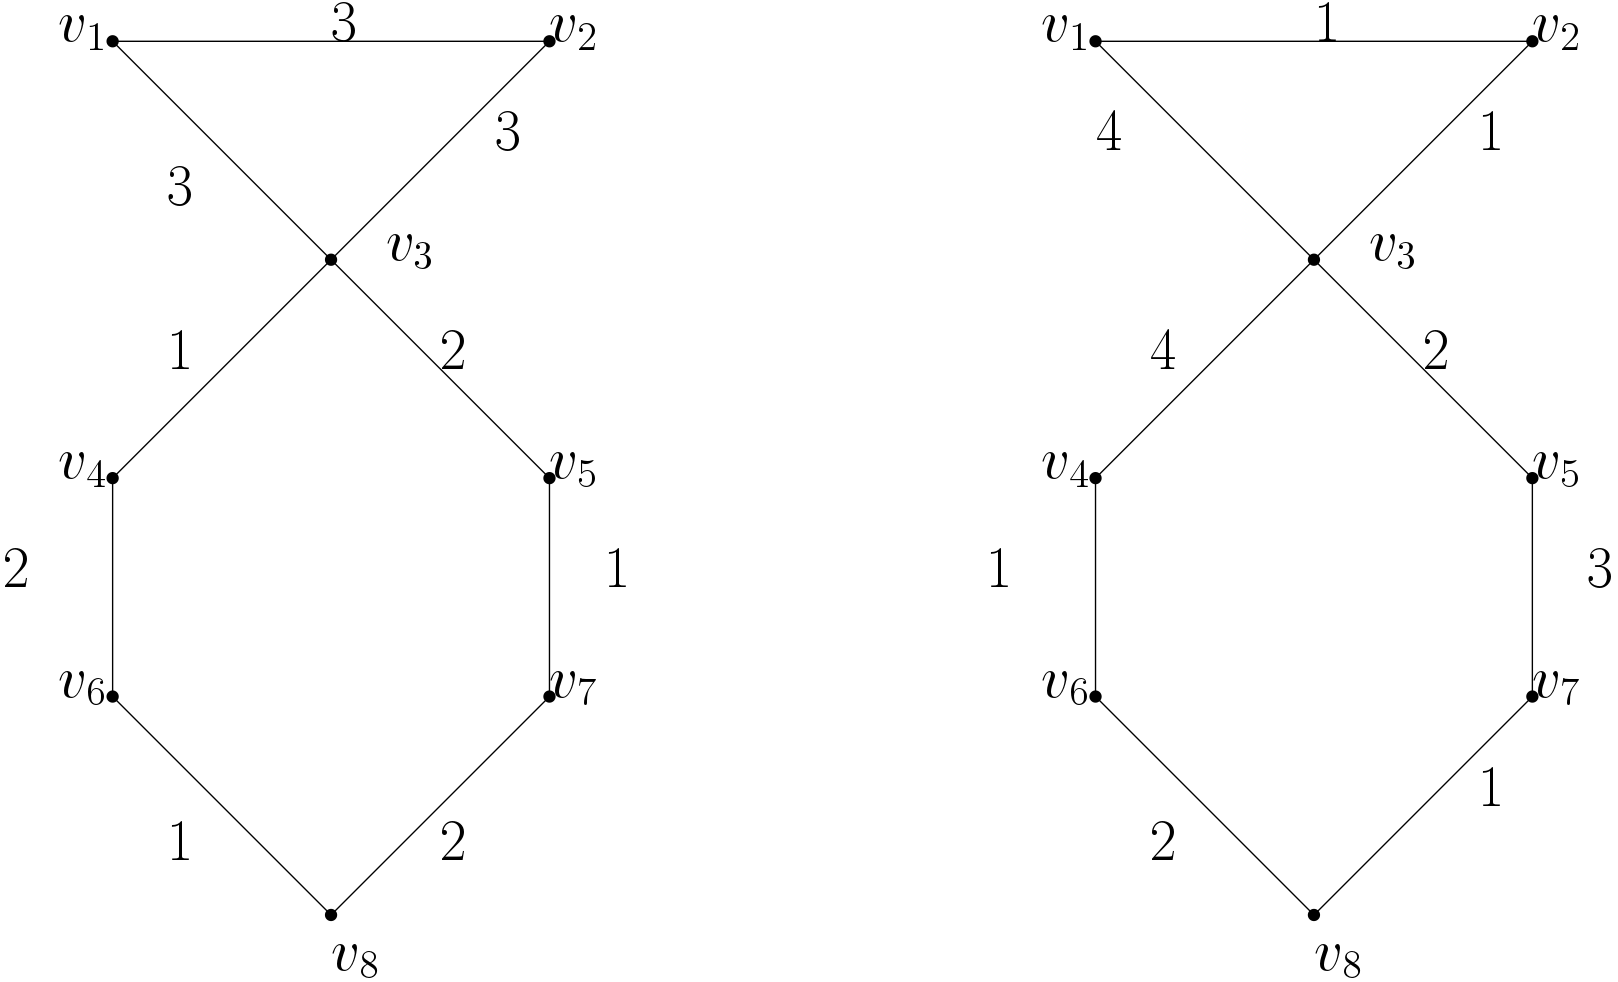
\includegraphics[width=1\linewidth]{figures/kpexample.png}
\end{center}
\caption{The label in left is a KP-labeling, while the one in right is not.}
\end{figure}
\begin{example}
Let us see two examples of edge labeling of the same graph $G$ as in Figure ~\ref{kpexample}.\newline
The label in the left side of figure satisfies condition $1$ as the edges of the triangle have the same label, also it satisfies condition $2$ as it can be checked that for arbitrary vertices $u$ and $v$ of $G$ with $d_G(u,v) \geq 2$ there exist different labels $i$ and $j$ which both appear on any induced $u$, $v$-path. Therefore the label in left is a KP-labeling.\newline
The label in right does not satisfy neither condition $1$ nor $2$, as the edges of the triangle do not have the same label, and also if we take vertices $v_5$ and $v_8$ then paths $P_1=v_5v_3v_4v_6v_8$ and $P_2=v_5v_7v_8$ have only one label in their intersecion.
\end{example}
\section{Induced subgraphs of Hamming Graphs}
Next we try to understand those Conditions 1 and 2 on cycle graphs and we infer the following result
\begin{lemma}\label{lemma:cyclenotunique}Let $G$ be a labeled graph fulfilling Condition 2 and let $C_k$, $k \geq 4$, be an induced cycle of $G$. Then every label of $C_k$ is present more than once on $C_k$.
\end{lemma}
\begin{proof}
The labels of a $u, v$-path of length $2$ on a $C_k$ are different, hence by Condition 2 those two labels should appear also along the other path. So for any label take two vertices $u$ and $v$ that have distance two and such that a $u,v$-path of length two contains the edge with that label, meaning that the label is present on both disjoin paths therefore the label is present more than once on $C_k$ 
\end{proof}
Before going to the main result we will need also the following lemma that tells us that we only need to check the induced paths.
\begin{lemma}\label{lemma:inducedpaths}Let $G$ be a labeled graph fulfilling Conditions 1 and 2 and let $u, v$ be vertices of $G$ with $d_G(u,v)\geq 2$. Then, if labels $i$ and $j$ appear on every induced $u, v$-path, they appear on every $u, v$-path.
\end{lemma}
\begin{proof}
Suppose that labels $i$ and $j$ appear on every induced \textsc{$u, v$-path} but not on every $u, v$-path. Let $P=x_1x_2...x_r, x_1=u$, with $x_r=v$, be a $u, v$-path of minimal length that does not contain both labels $i$ and $j$. Then $P$ is not induced since every induced path contains both labels, hence we have an edge between some non-consecutive vertices say $e=x_kx_l$ with $l-k>1$. We may assume that $e$ is chosen so that $l-k$ is as small as possible. By the minimality of $P$, the path $x_1x_2...x_kx_lx_{l+1}...x_r$ (which is shorter than $P$) contains both labels $i$ and $j$. Hence, the label of the edge $x_kx_l$ is either $i$ or $j$, otherwise $P$ would contain both labels $i$ and $j$. Assume without loss of generality that the label is $i$. Then, using minimality again, label $j$ appears on the path $x_1x_2...x_k$ or on $x_lx_{l+1}...x_r$ (note that it cannot happen that $k=1$ and $l=r$ as $d_G(u,v)\geq 2$). It follows that $i$ does not appear on the path $x_kx_{k+1}...x_l$. But then label $i$ appears only once on the cycle $C=x_kx_{k+1}...x_lx_k$. If $C$ is a triangle, we have a contradiction with Condition 1, otherwise with Lemma \ref{lemma:cyclenotunique}.
\end{proof}
If $G$ is a tree, then assigning a different label to each edge result in a labeling satisfying Conditions 1 and 2, hence in a $KP$-labeling. Note that every edge in a tree is a cut-edge. More generally, we can ask: which edges in a graph that has a $KP$-labeling can receive a unique label in some $KP$-labeling? This question is answered by the following result. 
\begin{proposition}
Let $G$ be a graph having a $KP$-labeling and let $e$ be an edge in $G$. Then $G$ has a $KP$-labeling in which $e$ receives a unique label if and only if $e$ is a cut-edge.
\end{proposition}

\begin{proof}
First we will show that if $e$ is a cut-edge then $G$ has a $KP$-labeling in which $e$ receives a unique label. Fix an arbitrary $KP$-labeling of G.\newline
Relabel edge $e$ with a new label, say $i$, not used before. We will show that the new labeling is also a $KP$-labeling. We need to verify the following two conditions:\newline
Condition 1: Every triangle is monochromatic.\newline Condition 1 holds, since $e$ is not part of any cycle (see Lemma \ref{cutedgecycle}) and therefore every triangle is still monochromatic.\newline
Condition 2: for every pair of distinct non-adjacent vertices $u,v$, there exist different labels $j$ and $k$ which both appear on every iduced $u,v$-path.\newline
To verify condition 2, note that any two $u,v$-paths either both contain edge $e$ or none (otherwise $e$ would be part of a cycle, but $e$ is a cut-edge)\newline
If none of the induced $u,v$-paths contains edge $e$ then the new $KP$-labeling still satisfies Condition 2 for the pair $u,v$ because of the original $KP$-labeling satisfied the condition for this pair.\newline
Otherwise all induced $u,v$-paths contain $e$, original label of $e$ be $i_0$. We consider/distinguish two cases:
\item[Case 1] If $i_0\in \{j,k\}$ then simply take the set $(\{j,k\}\setminus \{i_0\})\cup \{i\}$.
\item[Case 2] If $i_0\not\in \{j,k\}$ then simply take the set $\{j,k\}$.\newline
For the converse direction, suppose $G$ has a $KP$-labeling in which $e$ receives a unique label (by Corollary). Suppose for contradiction that $e$ is not a cut-edge. Then by Lemma \ref{cutedgecycle} $e$ is part of a cycle $C$. If $C$ is a triangle by Condition 1 and every edge of $C$ must have the same label as $e$, but then $e$ would not be labeled uniquely. Therefore $C$ cannot be triangle. 
Let $V(C)=\{v_1,v_2,...,v_p\}$ in cyclic order and without loss of generality $e=v_1v_2$. Let $u=v_1$ and $v=v_3$. Then since $e$ is labeled uniquely, the two induced paths forming a cycle from $u$ to $v$. These two paths cannot share any two labels so Condition 2 cannot hold, a contradiction. 
\end{proof}
\begin{theorem}\label{thm:mainkp}
Let $G$ be a connected graph. Then $G$ is an induced subgraph of a Hamming graph of dimension $d$ if and only if $G$ has a $d-KP$-labeling.
\end{theorem}
\begin{proof}
Let $G$ be an induced subgraph of $H=K_{n_1}\square K_{n_2}\square\cdots\square K_{n_d}$. To make things easier denote $p_i=p_{K_{n_i}}$, which is the projection of the complete graph $K_{n_i}$ of $H$ and also consider the labeling $E(G)$ induced by the color map $c$ of $H$. We will show that this labeling satisfies Conditions $1$ and $2$.\newline
Condition $1$ is clear. Indeed, if $u$, $v$, and $w$ induce a triangle, then they all lie in
the same layer of $H$ and by the alternative description of Hamming graphs we have that each pair is adjacent so they differ in exactly in one coordinate. Therefore color map $c$ will map those edges to the coordinate in which they differ and so the edges $uv$, $uw$, and $vw$ receive the same label.\newline
We next show that Condition $2$ is satisfied, too. Let $u$ and $v$ be two vertices of $G$ with $d_G(u,v)\geq 2$.
Suppose that there is no label that appears on all induced $u, v$-paths. Now if we see $u$ and $v$ as $d-tuples$ and we understand paths as changing coordinates and therefore $p_i(u)=p_i(v)$ for all $i$ because if we look at one induced path that does not have label $i$ that means than we never change the $i^{th}$ coordinate as we traverse this path and therefore the $i^{th}$ coordinates are the same, which implies $u=v$ contrary to $d_G(u,v)\geq 2$. Suppose now that all induced $u, v$-paths have exactly one label in common, say $i$. We have $p_j(u)=p_j(v)$ for all $j\neq i$ and consequently $p_i(u)\neq p_i(v)$ (since $u\neq v$). Vertices $p_i(u)$ and $p_i(v)$ are adjacent in $K_{n_i}$, since $K_{n_i}$ is a complete graph. Hence, $u$ and $v$ are adjacent in $H$ and therefore also in $G$ which is impossible.\newline
Conversely, let $\ell$ be a $d$-edge-labeling of $G$ that fulfills Conditions 1 and 2. Let $\mathcal{F}=\{F_1,F_2,\ldots F_d\}$ be the partition of $E(G)$ induced by $l$ and let $f$ be the quotient map of $G$ with respect to $\mathcal{F}$. We claim that $f$ embeds $G$ as an induced subgraph into $G=G/ F_1\square G/ F_2\square \ldots \square G/ F_d$.\newline
We show first that $f$ is one-to-one. Suppose that vertices $x$ and $y$ are not adjacent in $G$. Then by Condition 2 and Lemma ~\ref{lemma:inducedpaths}, there exist labels $i$ and $j$ such that on every $x, y$-path in $G$ we find labels $i$ and $j$. So $x$ and $y$ are in different components in both $G\backslash F_i$ and $G\backslash F_j$. Already the first fact assures that $f(x)\neq f(y)$. Let next $x$ and $y$ be adjacent vertices of $G$ and let $l(xy)=i$. We can see that $f_j(x)=f_j(y)$ for every $j\neq i$, they belong to same component they are adjacent, now let us take a look at $f_i$. Suppose that there exists an $x, y$-path $P=x_1x_2\ldots x_r$ in $G\backslash F_i$, where $x_1=x$ and $x_r=y$. We can assume that $P$ is shortest among all $x, y$-paths in $G\backslash F_i$. If $P$ is induced in $G-xy$ we have a contradiction with Condition 1 when $r=3$ since $P$ does not take the label $i$ (recall that $P$ is in $G\backslash F_i$) but a triangle will be formed with $xy$ and two edges in $P$. When $r>3$, we have and a contradiction with Lemma ~\ref{lemma:cyclenotunique} because $P+xy$ would form a cycle in which label $i$  is present only once. Thus $P$ is not induced in $G-xy$,
$r > 3$, and there are adjacent vertices $x_j$ and $x_k$ with $k > j+1$. By the minimality of $P$ we have $l(x_jx_k)=i$. We can select $j$ and $k$ such that $k- j$ is minimal among all such vertices $x_j$ and $x_k$. Then the cycle $C=x_jx_{j+1}\ldots x_{k-1}x_k$ is induced. If $C$ is a triangle we have a contradiction with Condition 1, otherwise we have a
contradiction with Lemma ~\ref{lemma:cyclenotunique}. Hence, we have shown that $f$ is one-to-one.\newline
Let $xy$ be an edge of $G$ with $l(xy)=i$. Then, by the above, $x$ and $y$ are in different components of $G\backslash F_i$. Moreover, they belong to the same component in any of the graphs $G\backslash F_j$ , for $j\neq i$. It follows that $f$ maps edges to edges and the claim is proved.\newline
Hence, $G=f(G)$ is an induced subgraph of $G\backslash F_1\square G\backslash F_2\square \ldots \square G\backslash F_k$. To complete the proof we show that $G$ is also an induced subgraph of the Hamming graph $k_{|G\backslash F_1|}\square K_{|G\backslash F_2|}\square \ldots \square K_{|G\backslash F_k|}$ :
Let $x$ and $y$ be non-adjacent vertices of $G$. Then, by the same reasoning as above, $x$ and $y$ are in different components of at least two graphs $G\backslash F_i$. It follows that $f(x)$ and $f(y)$ differ in at least two coordinates which remains valid after adding edges to the factor graphs.
\end{proof}
\begin{example} Let's see that $C_7$ is an induced subgraph of a Hamming graph and there exists a labeling of $C_7$ that fulfills Conditions $1$ and $2$.
\begin{figure}[h!]
\begin{center}
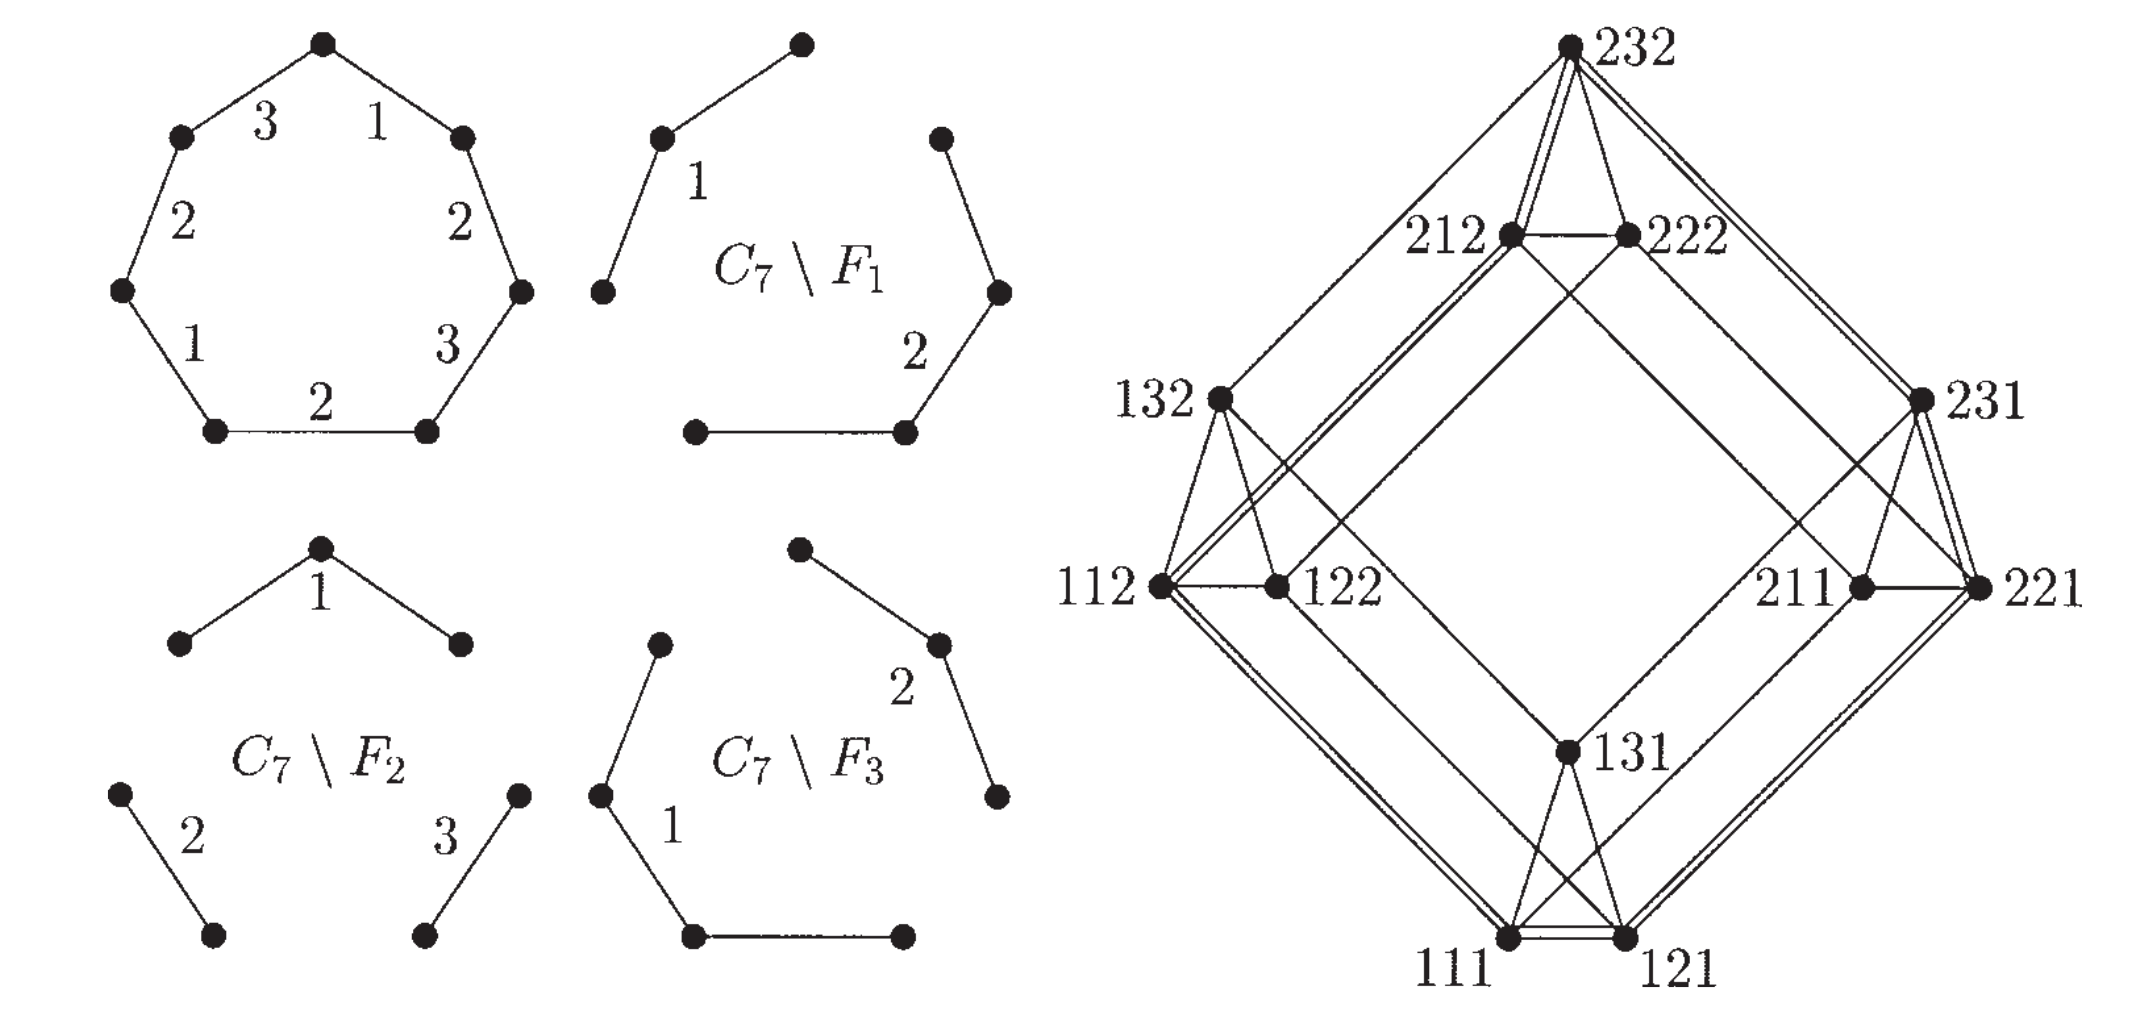
\includegraphics[width=1\linewidth]{figures/c_7inducedhamming.png}
\end{center}
\caption{$C_7$ as an induced subgraph of $K_2\square K_3\square K_2$}\label{fig:c7induced}
\end{figure}
\newline
$C_7$ is an induced subgraph of Hamming graph more specifically of $K_2\square K_3\square K_2$ in the Figure ~\ref{fig:c7induced} take cycle $(112,212,232,231,221,121,111)$ and using the color map $c$, edge $111,112$ gets label $3$, edge $112,212$ gets label $1$, edge $212,232$ gets label $2$, edge $232,231$ gets label $3$, edge $231,221$ gets label $2$, edge $221,121$ gets label $1$, edge $121,111$ gets label $2$. We can easily check that edges of a triangle have the same label (here there is no triangle which is fine) and let $u$ and $v$ be arbitrary vertices of $C_7$ with $d_{C_7}(u,v) \geq 2$. Then there exist different labels i and j which both appear on any induced u, v-path.\newline
$C_7$ has a labeling in which Conditions 1 and 2 hold as the first graph in Figure ~\ref{fig:c7induced}, now let's take a look at where does the map $f$ sends vertices of $C_7$. We follow the order clockwise from most top vertice, $f$ maps the first vertice to $112$, $f$ maps the second vertice to $212$, $f$ maps the third vertice to $232$, $f$ maps the fourth vertice to $231$, $f$ maps the fifth vertice to $221$,, $f$ maps the sixth vertice to $121$,, $f$ maps the seventh vertice to $111$ and as we can see $G=f(G)$ and induced subgraph of $K_2\square K_3\square K_2$
\end{example}
Note that the quotient graphs obtained in the proof of Theorem ~\ref{thm:mainkp} need not be complete. For instance, consider the path $P_4$ together with the labeling 1, 2, 1 as we get $G\backslash F_1=P_3$ and $G\backslash F_2=K_2$.
\chapter{Cartesian dimension}
Given a positive integer $d$, a $d$-realization of a graph $G=(V,E)$ is an injective mapping $\varphi_G:V\rightarrow \mathbb{R}^d$ such that two vertices $u, v \in V$ are adjacent if and only if $\varphi G(u)$ and $\varphi G(v)$ differ in exactly one coordinate. A graph $G$ is said to be $d$-realizable if it has a $d$-realization. Note that $G$ is $d$-realizable if and only if $G$ has a $d$-realization $\varphi_G : V \rightarrow \mathbb{N}^d$ or any large enough set of dimension $d$ since $V(G)$ is countable.\newline
Any graph that has a $d$-realization, it has also a $d+1$-realization (simply add one coordinate equal to $0$). Which naturally leads to a definition: the Cartesian dimension of a graph $G = (V, E)$, denoted $Cdim(G)$, is defined as the minimum non-negative integer $d$ such that $G$ is $d$-realizable, if such an integer exists, and $\infty$, otherwise. (Note that $K_1$ is the only graph of Cartesian dimension 0.)\newline

For a graph $G$ to have Cartesian dimension $1$ it must have a $1$-realization, or in other words you can map all the vertices of the graph to $\mathbb{R}$ and becuase the map has to be injective every vertice is mapped to different real number but every two vertice differ in exactly one coordinate which makes them adjacent, therefore the only graphs of Cartesian dimension $1$ are complete graphs of order at least $2$.

\begin{example}
$C_6$ has Cartesian dimension $2$, indeed since it is not a complete graph it cannot have dimension $1$, and we find a $2-realization$ of $C_6$ with vertex set $V=\{v_1,v_2,v_3,v_4,v_5,v_6\}$ and edge set $E=\{v_1v_2,v_2v_3,v_3v_4,v_4v_5,v_5v_6,v_6v_1\}$ by map defining $\varphi_{C_7}:V\rightarrow \mathbb{R}^2$ with $\varphi(v_1)=(1,1)$, $\varphi(v_1)=(1,1)$, $\varphi(v_2)=(3,1)$, $\varphi(v_3)=(3,3)$, $\varphi(v_4)=(2,3)$, $\varphi(v_5)=(2,2)$ and $\varphi(v_1)=(1,2)$. An easy check shows that indeed for any edge the corresponding values of $\varphi$ differ in exactly one coordinate.
\begin{figure}[h]
\begin{center}
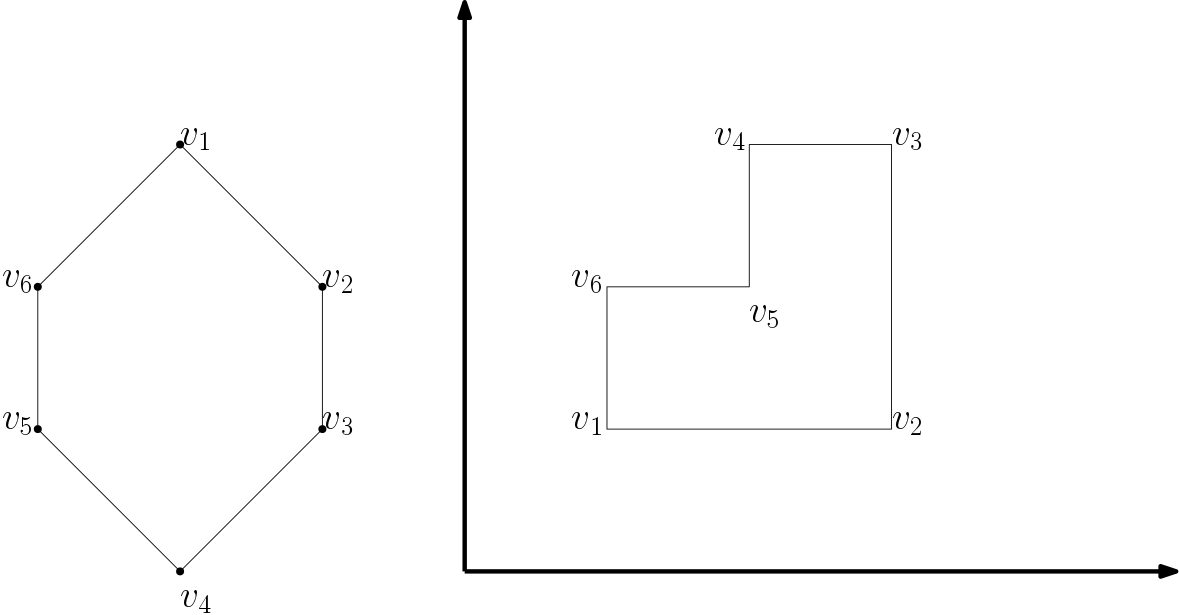
\includegraphics[width=1\linewidth]{figures/c_62real.png}
\end{center}
\caption{A $2$-realization of $C_6$}
\end{figure}
\end{example} 

\begin{lemma}\label{diamondfreecliques}
If graph $G$ is diamond-free then any two cliques of $G$ intersect in at most one vertex.
\end{lemma}
\begin{proof}
Suppose cliques $A_1$ and $A_2$ intersect in at least two vertices say $v_1, v_2$. Becuase $A_1$ is maximal clique there is some vertice $v_3$ other than $v_1,v_2$ in $A_1$ but not in $A_2$ and since $A_1$ is clique we have that $v_1,v_2,v_3$ form a triangle, similarly there exists $v_4$ in $A_2$ but not in $A_1$ such that $v_1,v_2,v_4$ form triangle. But all together $v_1,v_2,v_3,v_4$ form a diamond, a contradiction with $G$ being diamond-free.
\end{proof}

\begin{theorem}
For every graph G, the following conditions are equivalent:
\begin{enumerate}
\item $Cdim(G)\leq 2$.
\item $G$ is the line graph of a bipartite graph.
\item $G$ is diamond-free and $K(G)$ is bipartite.
\item $G$ is \{claw, diamond, $C_5$ , $C_7$ , ...\}-free.
\end{enumerate}
\end{theorem}

\begin{proof}
$(1)\implies(4)$ We show that none of those graphs in (4) can be an induced subgraph of a graph with $Cdim(G)\leq 2$. $Cdim(G)$ cannot be equal to $1$ since only complete graph with Cartesian dimension $1$. Now suppose it $Cdim(G)=2$.
\newline First let's show for diamond. Suppose G has diamond as induced subgraph with vertex set $V(G)=\{v_1,v_2,v_3,v_4\}$ and edge set $E(G)=\{v_1v_2,v_1v_3,v_2v_3,v_2v_4,v_3v_4\}$, now because $v_1$, $v_2$ and $v_3$ is complete graph on $3$ vertices all three together differ in one coordinate, similarly for $v_2$, $v_3$ and $v_4$ so it follows that also $v_1$ and $v_4$ differ only in one coordinate but they are not adjacent.
\newline Next suppose G has claw as induced subgraph with vertex set $V(G)=\{v_1,v_2,v_3,v_4\}$ and edge set $E(G)=\{v_1v_2,v_1v_3,v_1v_4\}$ and w.l.o.g. assume that assume that $\varphi_G(v_1)$ differs only in first coordinate with $\varphi_G(v_2)$ and because $v_2$ and $v_3$ are not adjacent then $\varphi_G(v_1)$ and $\varphi_G(v_3)$ must differ only in second coordinate. Which bring us to $v_4$, because $v_1$ and $v_4$ are adjacent they must differ only one coordinate, but either coordinate is not good as would  imply adjacency between $v_4$ and $v_2$ or $v_4$ and $v_3$ but there is no edge among them.
\newline And finally for odd-cycle larger than 3. Let the vertex set be $V(G)=\{v_1,v_2,...,v_n\}$ with edge set $E(G)=\{v_1v_2,v_2v_3,\ldots v_nv_1\}$ and notice that since there is no triangle no three vertices lie in same line so if we color map define in the section ~\ref{kp-labeling-section} then by by following the cycle we alternate by colors $1$ and $2$, but to close the cycle it must be followed by two different colors but cycle is odd so it is not possible.\newline
$(4)\implies (3)$ We only need to show that $K(G)$ is not bipartite which is equivalent that $K(G)$ has an odd cycle. Suppose it has length greater than $3$, first note that no three cliques(vertices in $K(G)$) share one vertice as then a claw would be form in $G$ but $G$ is claw-free, so we form an odd cycle by following the common vertice of cliques of size greater than $3$ but $G$ is $\{C_5,C_7,\ldots\}$-free, therefore $K(G)$ has a cycle of length $3$. Now if all three cliques have a vertice in common then we can form a claw because those cliques are maximal so there exist some vertex that other cliques don't have. Let those cliques that form a triangle be $A_1,A_2,A_3$ and the common vertex of $A_1,A_2$ be $v_1$, $A_2,A_3$ be $v_2$ and $A_3,A_1$ be $v_3$, because $v_1$ and $v_2$ are in $A_2$ they are adjacent, similiar for others. Notice that one of the cliques must have another vertex $v_4$ other than $v_1,v_2,v_3$ otherwise $K(G)$ would be just a vertex. Now w.l.o.g. say $v_4\in A_1$ then we have another triangle with $v_1,v_3\in A_1$, which all together $v_1,v_2,v_3,v_4$ forms a diamond but $G$ is diamond-free which leads to a contradiction, therefore $K(G)$ is bipartite.\newline 
$(3)\implies (1)$ If $G$ is complete then we know that $Cdim(G)=1$, suppose $G$ is not complete. Since $K(G)$ is bipartite we color vertices with two colors in natural way. Map vertices of $G$ in $\mathbb{R}^2$ by placing cliques of $G$ having one color on vertical lines and cliques having the other color on horizontal lines. By Lemma ~\ref{diamondfreecliques}, no two vertices are mapped to same point.
\newline
$(1)\iff (2)$ Given a bipartite graph $H$ such that $L(H)=G$, construct the adjacency matrix $A$. Mark points in $\mathbb{R}^2$ at $(i, j)$ iff $a_{ij} = 1$ in uppertriangle matrix of $A$. It is immediate that one can map vertex ${i,j}\in G$ to $(i,j)$ where $i<j$ and notice that this defines a one to one mapping and if two vertices are adjacent in $G$ then they will defer in exactly on coordinate. This shows that $Cdim(G)\leq 2$ as we found a $2$-realization.\newline
Since G can be realized with vertices only at positive integral points (the map $\varphi_G$ can be defined to $\mathbb{N}^d$), the proof works in reverse.
\end{proof}

\begin{lemma}\label{xyv adjacent}
Let $G$ be a d-realizable graph. Let $v$ be a vertex adjacent to vertices $x$ and $y$. Then $x$ and $y$ are adjacent if and only if they differ from $v$ in the same coordinate.
\end{lemma}
\begin{proof}
($\implies$) If $x$ and $y$ are adjacent then they differ in exactly one coordinate say in $k$th coordinate. Also say $v$ differs to $x$ exactly in $i$th coordinate and to $y$ in $j$th coordinate. Now suppose $x$ and $y$ don't differ from $v$ in the same coordinate which means that $i\neq j$, also note that $k$ cannot be equal to both $i$ and $j$ as this would imply $i=j$ so w.l.o.g. $k\neq j$. Now because $i\neq j$, the $j$th coordinate of $x$ is the same with $j$th coordinate of $v$ and therefore differs from $j$th coordinate of $y$, but also $k\neq j$ which means that $x$ and $y$ differ in more than one coordinate which contradicts the fact that $x$ and $y$ are adjacent.\newline
($\impliedby$) If they differ from $v$ in the same coordinate and because both of them are adjacent to $v$ then it means that they differ in exactly that coordinate which they differ with $v$, i.e. in one coordinate therefore they are adjacent.
\end{proof}

\begin{theorem}\label{d-realizable-free}
Every d-realizable graph is \{$K_{1,d+1}$ , diamond,
$K_{2,3}$ , $C_5$ \}-free.
\end{theorem} 
\begin{proof}
\textit{For $K_{1,d+1}:$} Suppose $v$ is the hub (the vertex with largest degree) of an induced $K_{1,d+1}$. Then $v$ differs from $n+1$ neighbors in different coordinates by Lemma ~\ref{xyv adjacent}, but there are only $n$ coordinates.\newline
\textit{For diamond:} If $v_1$, $v_2$, $x$ and $y$ are vertices of an induced diamond with $v_1$ and $v_2$ the vertices of degree $2$, then, invoking the Lemma ~\ref{xyv adjacent} we see that $v_1$ differs from $x$ and $y$ in the same coordinate. Similarly $v_2$ diifers from $x$ and $y$ in the same coordinate. Hence $v_1$ and $v_2$ differ from $x$ and $y$ in the same coordinate, and thus either $x=y$ or $x$ is adjacent to $y$.\newline
\textit{For $K_{2,3}$:} Let $x$ and $y$ be adjacent to all $v_1$,$v_2$,$v_3$ in an induced $K_{2,3}$. Then by Lemma ~\ref{xyv adjacent}, $v_1$,$v_2$, $v_3$ differ from $x$ in $3$ distinct coordinates. We assume that coordinates of $x$ are zeros. Then $y$ is at a distance of $2$ from x, so $y$ has $2$ non-zero coordinates. Hence $y$ has a zero in coordinate where either $v_1$,$v_2$ or $v_3$ is non-zero, and it follows that $y$ differs from one of these $3$ vertices in $3$ coordinates, and is therefore not adjacent to that vertex.\newline
\textit{For $C_5$:} Let $v_1$,$v_2$,$v_3$,$v_4$,$v_5$ be the vertices of a $5$-cycle in cyclic order. We assume that the coordinates of $v_1$ are all zeros.
$$v_1=(0,0,0,\ldots)$$
W.l.o.g. we can say
$$v_2=(\alpha,0,0,\ldots)$$
By the Lemma ~\ref{xyv adjacent} w.l.o.g.
$$v_3=(\alpha,\beta,0,0,\ldots)$$
Now if $v_4$ differed from $v_3$ in any coordinate other than the first two, $v_4$ would be at a distance at least $3$ from $v_1$ and it would be impossible to find $v_5$ to complete the $5$-cycle. Hence $v_4$ differs from $v_3$ in one of the first 2 coordinates. If 
$$v_4=(\alpha,\gamma,0,0,\ldots)$$
then $v_4$ is adjacent to $v_2$. Hence
$$v_4=(\delta,\beta,0,0,\ldots)$$
and the only choice for $v_5$ are
$$(\delta,0,0,0,\ldots)$$
and 
$$(0,\beta,0,0,\ldots)$$
The first of these is adjacent to $v_2$ and second is adjacent to $v_3$
 
\end{proof}

Staton and Wingard

Next we see the relation between $KP$-labeling and Cartesian dimension:
 \begin{theorem}[Klav\v zar and Peterin 2005]\label{cdim<kp}
For every connected graph G and a positive integer d, we have $Cdim(G) \leq d$ if and only if $G$ has a d-KP-labeling.
\end{theorem}

We take a closer look at 3-dimensional case and present two results both are related to the Klav\v zar-Peterin characterization which is needed for hardness proof for recognizing 3-realizable graphs developed in paper (here reference paper of Prof Martin).\newline
In the first result, we will see that the defining properties of a 3-KP-labeling are satisfied for a graph as soon as they are satisfied for the family of all its induced subgraphs isomorphic to a cycle or to a $P_3$.

\begin{theorem}\label{3-edge-label}
Let $G$ be a graph. A 3-edge-labeling of $G$ is a KP-labeling if and only if it satisfies the following two conditions:\newline
\textbf{Condition 3}: for every induced cycle $C$ of $G$, the restriction of the labeling to $E(C)$ is
a KP-labeling of $C$.\newline
\textbf{Condition 4}: no induced $P_3$ is monochromatic.
\end{theorem}

\begin{proof}
Let us start by showing the necessity of the two conditions. If $G$ is 3-KP-labeling and $H$ is an induced subgraph of $G$, then the restriction of the labeling to $E(H)$ is a 3-KP-labeling of $H$ because every path in $H$ is still a path in $G$, hence Condition 3 is necessary. Condition 4 follows from the fact that every induced $P_3$ must contain two different labels since it is a path itself.\newline 
Now we prove the sufficiency. For Condition 1 it is needed to show that every triangle is monochromatic but from Condition 3 we know that for every induced triangle of $G$, the restriction to edges, which is the same triangle is KP-labeling but triangle is KP-labeling if and only if it is monochromatic.\newline
Now let's show that Condition 2 also holds by contradiction.\newline
Suppose  that there is a 3-edge-labeling $l:E(G)\rightarrow \{1,2,3\}$ satisfying Conditions 3 and 4, but not Condition 2. Singe Condition 2 does not hold in $G$, it means that $G$ contains two different induced paths of length at least two, say $P$ and $Q$, intersecting at their endpoints $u$ and $v$, such that no pair of different labels appears on both $P$ and $Q$.\newline
Due to Condition 4, on each of the paths $P$ and $Q$ at least two different labels appear. Since no pair of different labels appears on both $P$ and $Q$, we may assume that $P$ and $Q$ take alternatingly labels 1, 2 and 1, 3, respectively. Moreover, assume that $P$ and $Q$ were chosen so as to minimize $|V(P)|+|V(Q)|$.\newline
We continue with definition to facilitate our way in the proof. Given a path $R$ and two of its vertices $x$ and $y$, denote by $R_{xy}$ the subpath of $R$ between
$x$ and $y$, and by $V(R)^{-xy}$ the set $V(R)\backslash \{x,y\}$. Also, say a path is $k$-labeled if exactly $k$
different labels appear on its edges.\newline
We claim that $V_P^{−uv} \cap V_Q^{−uv} = \emptyset$. Suppose that there is something in intersection, $w\in V_P^{−uv} \cap V_Q^{−uv}$. First we see that $P_uw$ and $Q_uw$ cannot be 1-labeled because of Condition 4 none of the paths can have length more than 2, which must follow that $u$ and $w$ are adjacent, but this is in contradiction with minimality of $|V(P)|+|V(Q)|$. So it must be that $P_uw$ and $Q_uw$ are 2-labeled. Since there are only 3 labels it must be the case that $P_{uw}\cup Q_{uw}$ would be 3-labeled, again contrandiction with minimality of $|V(P)|+|V(Q)|$ as we found a path with 3 labels satisfying what we need. \newline
We add also some definitions, which will help us. For $t \in \{u, v\}$ and $xy \in E(G)$ with $(x, y) \in V_P^{−uv} \times V_Q^{−uv}$, a cycle $C = P_{tx}-xy-Q_{yt}$ such that either $P_{tx}-xy$ or $xy-Q_{yt}$ is an induced path will be called a $PQ$-cycle. Note that a
$P Q$-cycle cannot be 3-labeled: with out loss of generality say $P' = P_{tx} -xy$ was an induced path, then we can find a shorter path, namely the path $P'$ and $Q_{yt}$ would contradict minimality of $|V(P)|+|V(Q)|$.\newline
Let us investigate the cycle $C_0=P\cup Q$, from our assumption that not to labels appear in both paths $P,Q$, from Condition 3 we have in induced cycle, the restriction of the labeling to $E(C_0)$ is a KP-labeling of $C_0$ it must follow that $C_0$ is not an induced cycle as the restriction of the labeling to $E(C)$ is obviously not a KP-labeling of $C_0$. Let $xy$ be a chord in $C_0$ such that $\{x, y\} \cap \{u, v\} = \emptyset$ such that $x \in V (P )$ is closest to $u$(where the distance is measured
within $P$), and $y$ is the neighbor of $x$ in $Q$ closest to $v$ (where the distance is measured within $Q$). Now we observe two cycles that are formed, namely $C_1 = P_{ux}-xy-Q_{yu}$ and $C_2 = P_{vx} -xy-Q_{yv}$, because of how we selected $x$ and $y$ each of $C_1,C_2$ is either a $P Q$-cycle or a triangle, implying that neither of them is 3-labeled. If $C_1$ is monochromatic then, as $E(C_0) \subset E(C_1 ) \cup E(C_2)$ while $C_1$ and $C_2$ share the label of $xy$, it would follow that $C_2$ was 3-labeled, symmetricaly if $C_2$ was monochromatic. Thus, $C_1$ and $C_2$ are 2-labeled. \newline
As $C_1$ and $C_2$ are 2-labeled, they share exactly one label. By definition, any $P Q$-cycle contains a $P_3$ from either $P$ or $Q$, hence (recalling that $P$ and $Q$ alternate labels 1, 2 and 1, 3, respectively), $C_1$ and $C_2$ share label 1. Such is then the label of $xy$. However, one of the two edges incident to $x$ in $P$ is also labeled with 1, forming with $xy$ a monochromatic
induced $P_3$ (as part of either $C_1$ or $C_2$), which contradicts Condition 4. 
\end{proof}

\begin{example}
We will see an example where the Theorem \ref{3-edge-label} does not work for 4-edge-labeling. We find a graph satisfying Condition 3 and 4 but it is not a KP-labeling.\newline
Take the graph $G$ with 4 paths of length 6 sharing only the endpoints vertices, say $u$ and $v$. Label the paths in following way:\newline
\textit{path 1: 1, 2, 3, 1, 2, 3}\newline
\textit{path 2: 2, 3, 4, 2, 3, 4}\newline
\textit{path 3: 3, 4, 1, 3, 4, 1}\newline
\textit{path 4: 4, 1, 2, 4, 1, 2}\newline
A quick check can show that every induced cycle is a KP-labeling and also no $P_3$ is monochromatic, which means that Condition 3 and 4 are satisfied. However if we check whether this labeling is a KP-labeling of $G$, taking non-adjacent vertices $u$ and $v$, we can see that each pair of the 4 paths share exactly 2 labels, but from pingeonhole principle we cannot find labels $i$ and $j$ which both appear on any induced $u, v$-path.\newline
This example can be generalized that Theorem \ref{3-edge-label} does not work for any $d>3$.  
\begin{figure}[h]
\begin{center}
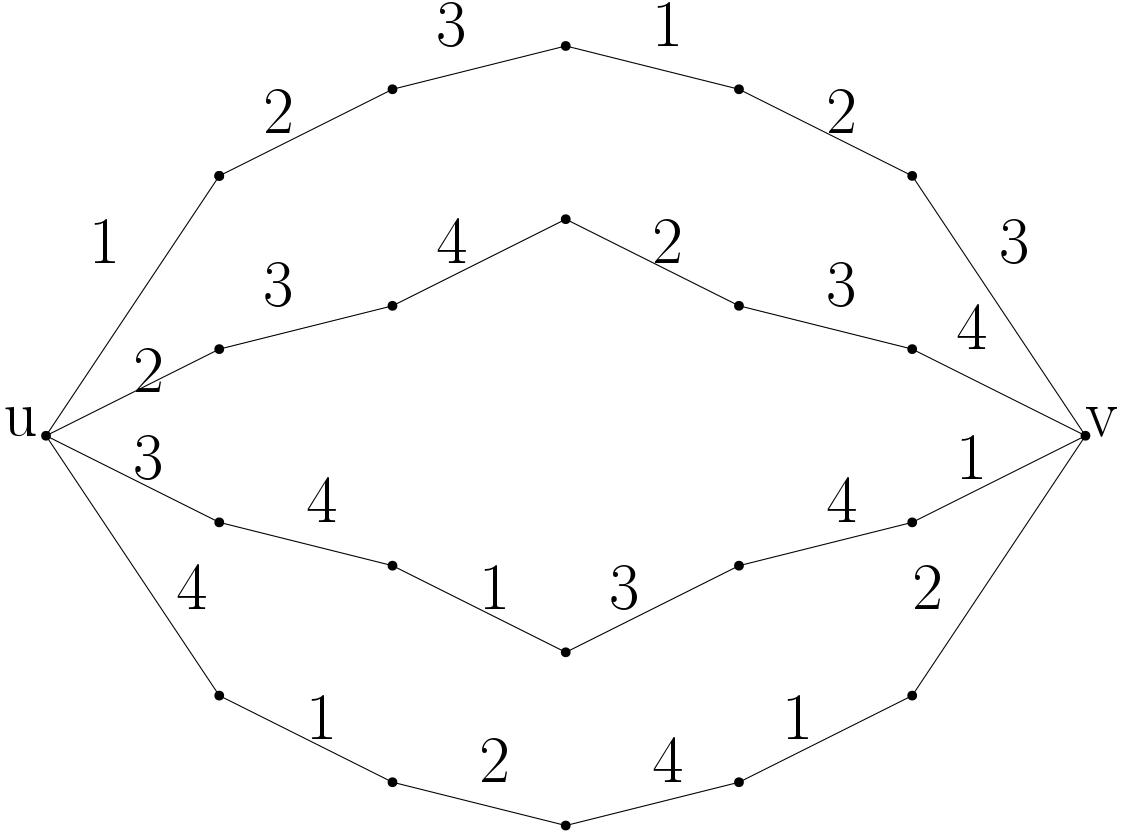
\includegraphics[width=0.6\linewidth]{figures/d4.png}
\end{center}
\caption{Counterexample of Theorem \ref{3-edge-label} for 4-edge-labeling}
\end{figure}
\end{example}
From Condition 1 we know that every 3-KP-labeling of 3-cycle is constant(monochromatic). The folliwing result analyzes longer cycles.
\begin{lemma}
Let $C$ be a cycle of length at least 4. A 3-edge-coloring of $C$ with colors 1, 2, 3 is a KP-labeling if and only if
\begin{itemize}
\item either it is a 2-edge-coloring of $C$, or
\item possibly after permuting the labels 1, 2, 3, cycle $C$ contains a cyclically ordered sequence
of 6 distinct (not necessarily consecutive) edges labeled 1, 2, 3, 1, 2, 3, respectively. 
\end{itemize}
\end{lemma}

\begin{proof}
($\implies$) If the label is 2-edge-coloring then it follows, otherwise suppose that $C$ is KP-labeled with an edge-coloring using colors 1,2 and 3 so that all three labels appear on $E(C)$. Fix a cyclic order $\sigma$ of the edges of $C$. Without loss of generality, $C$ has a pair of consecutive edges in $\sigma$, say $e_1$ and $e_2$, that are labeled 1 and 2 respectively. Each label must appear at least twice on $C$, since otherwise the endpoints of a path formed by two consecutive edges containing a label that appears exactly once would violate Condition 2. Then, the sequence 1,2,3,3 must appear as a sequence of the labels of edges in order $\sigma$, we stress it here from the lemma that this order is not necessarily consecutive (we could have something like 1,2,3,1,2,1,2,3). Let $P$ be the maximal subpath of $C$ containing $e_1$ and $e_2$ having no edge labeled 3, and let $e$ and $e'$ be the two edges of $E(C)\backslash E(P)$ incident to an edge in $P$. By the maximality of $P$, edges $e$ and $e'$ are labeled 3 and, since each each label appears twice they must be distinct. Let $P'$ be the subpath of $C$ formed by the edges not in $E(P)\cup \{ e,e'\}$. Since $P$ has only labels 1 and 2, in order not to violate Condition 2 both of them must appear in $E(C)\backslash E(P)$ and since $e,e' \in E(C)\backslash E(P)$ are labeled 3, it follows that labels 1,2 must appear in $E(P')$. If labels 1 and 2 appear in order $\sigma$ on $P'$ (not necessarily consecutively), we are done. Suppose then that all occurrences of 2 appear in $\sigma$ before all occurrences of 1 on $E(P')$. If on $P$ there is an occurrence of label 2 appearing (in $\sigma$) before an occurence of 1, we are done again. By way of contradiction  ,suppose that this is not the case, that is, suppose that all occurces of 1 appear (in $\sigma$) before all occurences of 2 on $P$. \newline
Then $C$ can be divided in two parts in such a way that the occurrences of 1 appear only in one part and the occurences of 2 in the other part, which will violate Condition 2.\newline
($\impliedby$) Since there are no triangles, Condition 1 is satisfied. \newline
If $C$ is 2-edge-labeled, then clearly Condition 2 holds.\newline
Suppose now, without loss of generality, that $C$ contains a cyclically ordered sequence of 6 distinct (not necessarily consecutive) edges labeled 1, 2, 3, 1, 2, 3, respectively. Let $F$ denote a fixed set of 6 edges with the above property. Consider now an arbitrary pair $u,v$ of non -adjacent vertices of $C$. Let $P$ and $Q$ be the two $u,v-$subpaths of $C$. At least on of $P$ and $Q$, say $P$, contains at least three consecutive edges from $F$. Hence, any two distinct labels appearing on $Q$ will appear on every induced $u,v-$path. Since this is true for an arbitrary pair $u,v$ of nonadjacent verices, Condition 2 is satisfied.


\end{proof}

\subsection{Cartesian dimension of $P_i\square P_j$}
A two-dimensional grid graph is the Cartesian product two path graphs. The results below will demonstrate that when finding the exact Cartesian dimension of these graphs and for paths of length at least 3, the Cartesian dimension is equal for any pair of path graphs. To prove these results, we will use the Theorem \ref{cdim<kp} which shows the relation between Cartesian dimension and KP-labeling.\newline
\begin{theorem}
$Cdim(P_i \square P_j) = \left\{0,2,3,4\right\}$
\end{theorem}
\begin{proof}

 Without loss of generality, let us take $i\leq j$.\newline
\textit{Case 1} If $i=1$, then $P_1\square P_j=P_j$; if $j=1$ then $Cdim(P_i\square P_j)=0$;
\textit{Case 2} If $j=2$, then $Cdim(P_i\square P_j)=1$; and if $j\geq 2$, then $Cdim(P_i\square P_j)=2$
 .\newline 
If $i=2$ and $j=2$, then $Cdim(P_i\square P_j)=2$.
As a result, we write the following proposition
\newline
\textit{Case 3} If $j\geq 3$, from Theorem \ref{d-realizable-free}, we have that $Cdim(P_2\square P_j)\geq 3$, since $P_2 \square P_j$ has $K_{1,3}$ as induced subgraph.\newline
Next, we find a $KP$-labeling of the graph with 3 labels.
\begin{figure}[h]
\begin{center}
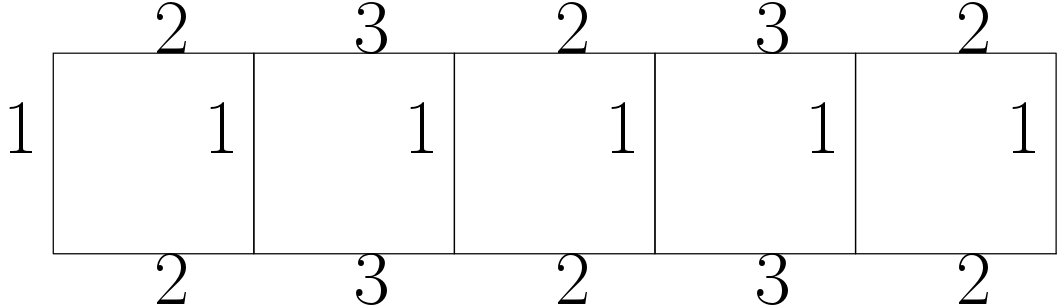
\includegraphics[width=0.6\linewidth]{figures/p_2sqp_j.png}
\end{center}
\caption{KP-labeling of $P_2\square P_6$}\label{fig:P_2sqP_6}
\end{figure}\newline
We label the copies of the first factor ($P_2$) with label 1 and both copies of $P_j$ the same by alternating between 2 and 3.
An example of how would we label $P_2\square P_6$ is shown in Figure \ref{fig:P_2sqP_6}.\newline
For any two nonadjacent vertices, $u$ and $v$, if they belong to a $C_4$, we take label 1 and the other label from set $\{2,3\}$ to satisfy Condition 2; otherwise take labels 2 and 3 for vertices, $u$ and $v$, when they do not belong to some $C_4$ and $u$ and $v$ are in different components when taking the partition of graph with respect to labels 2 or 3, meaning that the edges labeled with $i$ determine a cut-set, for $i$ in $\{2,3\}$.\newline
Therefore, this labeling is a KP-labeling and from Theorem \ref{cdim<kp}, we have that $Cdim(P_2\square P_j)\leq 3$.\newline
Combining both inequalities, we have that $Cdim(P_2\square P_j)=3$ if $j\geq 3$



Finally, we will look at the general case when $i\geq 3$.
\newline
\textit{Case 4} if $i\geq 3$, from Theorem \ref{d-realizable-free}, we have that $Cdim(P_i\square P_j)\geq 4$, since $P_i \square P_j$ has $K_{1,4}$ as induced subgraph.\newline
Next, we find a KP-labeling of the graph with 4 labels.
\begin{figure}[h]
\begin{center}
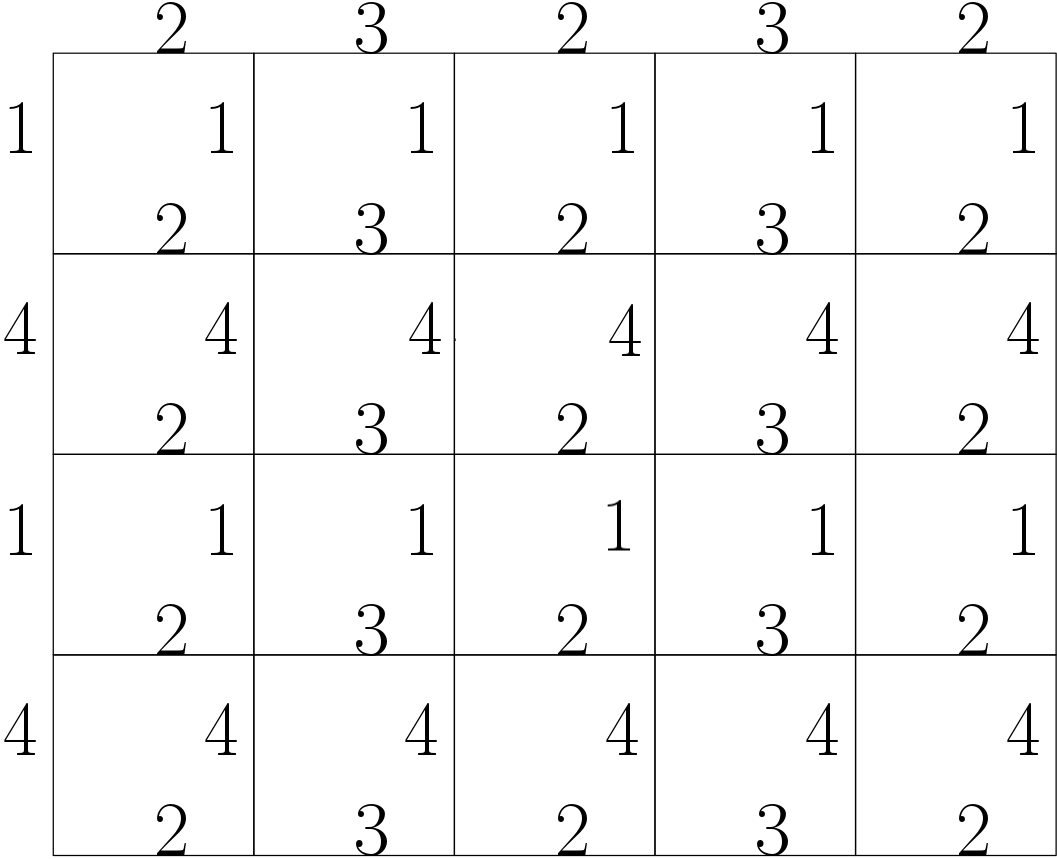
\includegraphics[width=0.6\linewidth]{figures/p_isqp_j.png}
\end{center}
\caption{KP-labeling of $P_5\square P_6$}
\end{figure}\newline
We label the copies of $P_i$ identically by alternating between 1 and 4; and the copies of $P_j$ identically by alternating between 2 and 3.\newline
For any two nonadjacent vertices, $u$ and $v$, when they belong to a $C_4$, we take the labels in this cycle. However, if any two nonadjacent vertices, $u$ with coordinates $(a,x)$ and $v$ with coordinates $(b,y)$, do not belong to a $C_4$, then either $d_{P_i}(a,b) \geq 2$ or $d_{P_j}(x,y) \ge 2$. If $d_{P_i}(a,b) \geq 2$, we take labels 2 and 3; otherwise, we take labels 1 and 4. Similarly to the previous proposition, vertices $u$ and $v$ would belong to different components when removing either of the choosen labels. 
 \newline
Therefore, this label is a KP-labeling and from Theorem \ref{cdim<kp}, we have that $Cdim(P_i\square P_j)\leq 4$.\newline
Combining both inequalities, we have that $Cdim(P_i\square P_j)=4$, if $i\geq 3$
\end{proof}

\chapter{Hamming dimesion}
Graph products offer a variety of possibilities to introduce the concept of a graph dimension. A classical result of Graham and Winkler \cite{Graham} shows that any graph can be canonically isometrically embedded into the Cartesian product of graphs. Knowing that, this embedding is unique among all irredundant isometric embeddings with respect to the largest possible number of factors, the latter numberis is defined to be the \textit{isometric dimension} of a graph. 
\newline The strong product $G\boxtimes H$ of graphs $G$ and $H$ is a graph such that the vertex set of $G\boxtimes H$ is the Cartesian product $V(G) \times V(H)$; and distinct vertices $(u,u')$ and $(v,v)$ are adjacent in $G\boxtimes  H$ if and only if $u = v$ and $u'$ is adjacent to $v'$, or $u' = v'$ and $u$ is adjacent to $v$, or $u$ is adjacent to $v$ and $u'$ is adjacent to $v'$. Back in 1938 Sch\" onberg \cite{Schonber} proved that every connected graph admits an isometric embedding into the strong product of paths. It is hence natural to define the \textit{strong isometric dimension}, $idim(G)$, of a graph $G$ as the least number $k$ such that $G$ embeds isometrically into the strong product of $k$ paths.\newline
David Eppstein consider the following representation problem: for which unweighted undirected graphs can be assigned integer coordinates in some $d$-dimensional space $Z^d$, such that the distance between two vertices in the graph is equal to the $L_1$-distance(taxicab) between their coordinates? Call the minimum possible dimension $d$ of such an embedding (if one exists) the \textit{lattice dimension} of the graph.\newline
The strong isometric dimension is universal in the sense that as soon as a graph is not the path graph, then its dimension is finite and bigger than 1. A similar conclusion can be stated for the so called direct dimension of a graph. On the other hand, for the most important graph product, the Cartesian one, no such universal dimension is known. While the isometric dimension is useful as soon as the dimension of a graph is more than 1, it was proved in \cite{Poljak} that for almost any graph its isometric dimension is 1. In
other words, for almost any graph $G$, the isometric dimension yields no new insight about $G$. Also, only
partial cubes, a special (although important) subclass of bipartite graphs, have finite lattice dimension.\newline

We say that a graph $G$ is an irredundant subgraph of $\square _iG_i$ if each $G_i$ has at least two vertices and any vertex of $G_i$ appears as a coordinate of some vertex of $G$.\newline
In order to significantly increase the number of graphs with a non-trivial dimension that comes from the Cartesian product of graphs Sandi Klav\v zar, Iztok Peterin and Sara Sabrina Zemlji\v c in \cite{Sandi}, defined the \textit{Hamming dimension} $Hdim(G )$ of a graph $G$ is introduced as the largest dimension of a Hamming graph into which $G$ embeds as an irredundant induced subgraph. If $G$ is not an induced subgraph of any Hamming graph we set $Hdim ( G ) = \infty$.\newline In Figure \ref{fig:c6hdim} is shown $C_6$ induced in two different Hamming graphs, $K_3\square K_3$ and $K_2\square K_2\square K_2$
\begin{figure}[h]
\begin{center}
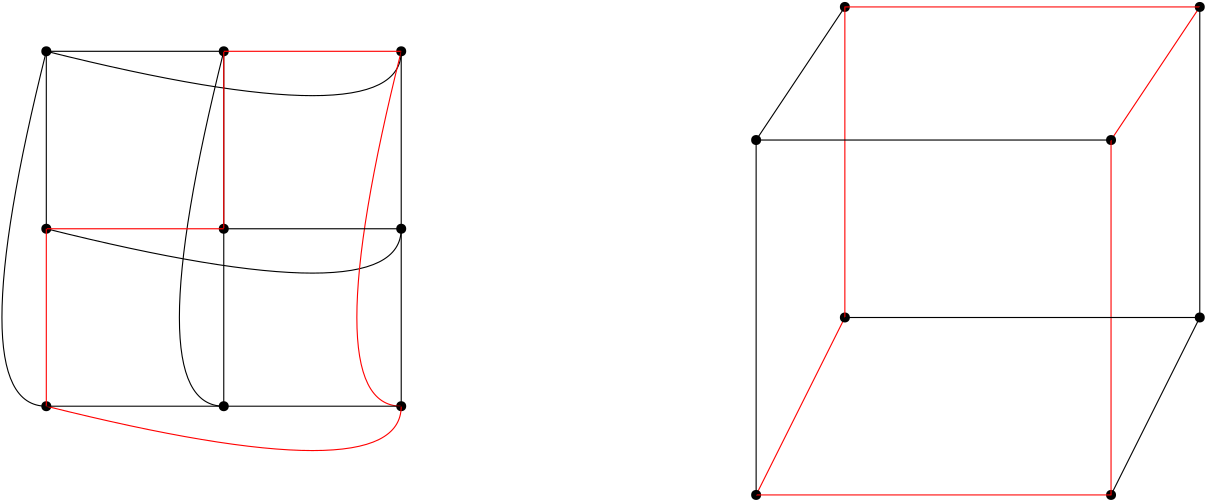
\includegraphics[width=1\linewidth]{figures/c_6hdim.png}
\end{center}
\caption{$C_6$ induced in $K_3\square K_3$ and $K_2\square K_2\square K_2$}\label{fig:c6hdim}
\end{figure}
Clearly, $Hdim ( G ) = 1$ if and only if $G$ is a complete graph. By Theorem \ref{thm:mainkp}, we can understand it as $Hdim ( G ) <\infty$ if and only if $G$ has a $d-KP$-labeling.
\section{Hamming dimension of Sierpiński graphs}
The general problem of determining the Hamming dimension of a graph seems very demanding, here we will study this concept on Sierpiński graphs. Roughly speaking, in \cite{Sandi}, they proved that all Sierpi\'nski graphs (except in the trivial cases) have Hamming dimension bigger than 1 and finite. On the other hand, all but base 3 Sierpi\'nski graphs have isometric dimension 1. Hence the Hamming dimension indeed significantly increases the number of graphs with a non-trivial Cartesian-like dimension.\newline
Graphs whose drawings can be viewed as approximations to the famous Sierpi\'nski triangle have been studied intensely in the past 25 years. The interest for these graphs comes from many different sources such as games like the Chinese rings or the Tower of Hanoi, topology, physics, the study of interconnection networks, and elsewhere.\newline
Sierpi\'nski graphs $S^{k}_n$ were studied for the first time in \cite{Sandi2}. In computer science, a very similar class of graphs (known as WK-recursive networks) was introduced earlier. The study in \cite{Sandi2} was motivated in part by the fact that for $k=3$ these graphs are isomorphic to the Tower of Hanoi graphs and in part by topological studies.\newline
The graphs $S^k_n$ were investigated from numerous points of view, we recall some of them. These graphs contain unique 1-perfect codes. Metric properties of Sierpi\'nski graphs were investigated in \cite{Andreas}. To
determine the chromatic number of these graphs is easy, while in \cite{Andreas2} it is proved that they are in
edge- and total coloring class 1, except those isomorphic to a complete graph of odd or even order, respectively.\newline
The Sierpi\'nski graph $S^k_n$ , $k,n\geq 1$, is defined on the vertex set $\{ 1,\ldots,k \}^n$ , two different vertices $u = ( u 1 ,\ldots, u_n )$ and $v = (v 1 ,\ldots , v_n )$ being adjacent if and only if there exists an $h \in \{ 1 , \ldots, n \}$ such that
\begin{enumerate}[label=(\roman*)]
\item $u_t = v_t$ , for $t = 1 ,\ldots , h − 1$;
\item $u_h \neq v_h$ ; and
\item $u_t = v_h$ and $v t = u h$ for $t = h+ 1 ,\ldots, n$.
\end{enumerate}
An example of Sierpi\'nski Graph is shown in Figure \ref{fig:spierpinski}.
\begin{figure}[h]
\begin{center}
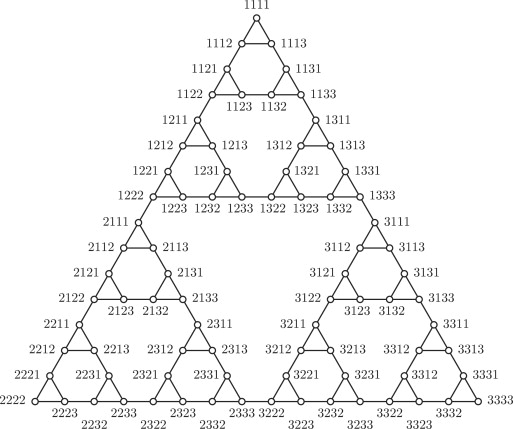
\includegraphics[width=1\linewidth]{figures/sierpinski.png}
\end{center}
\caption{The Sierpi\'nski graph $S^3_4$}\label{fig:spierpinski}
\end{figure}
We will use abbreviation $\langle u_1,\ldots, u_n \rangle$ for $(u_1,\ldots, u_n)$ and in figures will use the short version $u_1\ldots u_n$. \newline
A vertex of the form $\langle ii \ldots i \rangle$ of $S^k_n$ is called an extreme vertex. Note that $S^k_n$ contains $k$ extreme vertices and that $| V ( S^k_n )| = k^n$.




 \begin{thebibliography}{99}
\thispagestyle{fancy}

\bibitem{Graham}
  \articleInJournalManyAuthors
    {R.L. Graham and P.M. Winkler}
    {On isometric embeddings of graphs}
   {rans.Amer. Math. Soc.}{288}
   {1985}{527--536}

\bibitem{Schonber}
\articleInJournalOneAuthor
    {I.J. Schonber}
    {Metric spaces and positive definite functions}
   {Trans. Amer.Math. Soc.}{44}
   {1938}{522--536}

\bibitem{David}
\articleInJournalOneAuthor
    {David Eppstein}
    {The lattice dimension of a graph}
   {European Journal of Combinatorics}{26}
   {2005}{585--592} 

\bibitem{Poljak}
  \articleInJournalManyAuthors
    {S. Poljak and A. Pultr}
    {Representing graphs by means of strong and weakproducts}
   {Comment. Math. Univ. Carolin.}{22}
   {1981}{449--466}  
   
\bibitem{Sandi}
  \articleInJournalManyAuthors
    {Sandi Klav\v zar, Iztok Peterin and Sara Sabrina Zemlji\v c}
    {Hamming dimension of a graph—The case of Sierpi\'nski graphs}
   {European Journal of Combinatorics}{34}
   {2013}{460--473}

\bibitem{Sandi2}
  \articleInJournalManyAuthors
    {Sandi Klav\v zar, Uro\v s Milutinovi\' c}
    {Graphs $S(n, k)$ and a Variant of the Tower of Hanoi Problem}
   {Czechoslovak Mathematical Journal}{47}
   {1997}{95--104}

\bibitem{Andreas}
  \articleInJournalManyAuthors
    {Andreas M. Hinz,Daniele Parisse}
    {The Average Eccentricity of Sierpiński Graphs}
   {Graphs and Combinatorics}{28}
   {2012}{671--686}
   
\bibitem{Andreas2}
  \articleInJournalManyAuthors
    {Andreas M. Hinz,Daniele Parisse}
    {Coloring Hanoi and Sierpiński graphs}
   {Discrete Mathematics}{312}
   {2012}{1521--1535}   

% There has to be an empty line here so that the page numbers of citations are properly displayed.
\end{thebibliography}
\newpage

%%%%%%%%%%%%%%%%%%%%%%%%%%%%%%%%%%%% Appendices %%%%%%%%%%%%%%%%%%%%%%%%%%%%%%%%%%%%%

\pagestyle{fancyplain}
\vspace*{\fill}
     \begin{center}
          \bf{\Huge{Appendices}}
     \end{center}
\vspace*{\fill}
\thispagestyle{fancy}

\appendix
\thispagestyle{empty}
\pagenumbering{gobble}

\addtocontents{toc}{\setcounter{tocdepth}{-1}}
\appendices{A Title of First Appendix}
\chapter{Title of First Appendix}
\thispagestyle{empty}
Here we add the first appendix.

% Be careful:
% the command
% \thispagestyle{empty}
% has to be present on every page of each appendix (so that the document header is not displayed)

\appendices{B Title of Second Appendix}
\chapter{Title of Second Appendix}
\thispagestyle{empty}
Here we add the second appendix.

% Be careful:
% the command
% \thispagestyle{empty}
% has to be present on every page of each appendix (so that the document header is not displayed)

\addtocontents{toc}{\setcounter{tocdepth}{2}}
\end{document}
